Before delving further into the approach taken for the indexing and retrieval of the documents, we shall analyze the documents contained in the APIs.guru dataset. \\ \\
During this phase, we had to visualize the semantic relationship of the documents.
To do so, we embedded (Subsection~\ref{subsec:document-embedding}) the documents in 512 dimensions.
Once embedded, we performed a dimensionality reduction using t-SNE (Subsection~\ref{subsec:t-sne-plots}).
At this point we added the third dimension representing the category of the document, and plotted the points.
The category of the API specification is taken from the \verb|info.x-apisguru-categories| tag manually assinged by APIs.guru. \\ \\
The aforementioned steps produce the result depicted in Figure~\ref{fig:documents-plot}.
\begin{figure}%
    \centering
    \subfloat[\centering Documents Color-Coded by Category] {{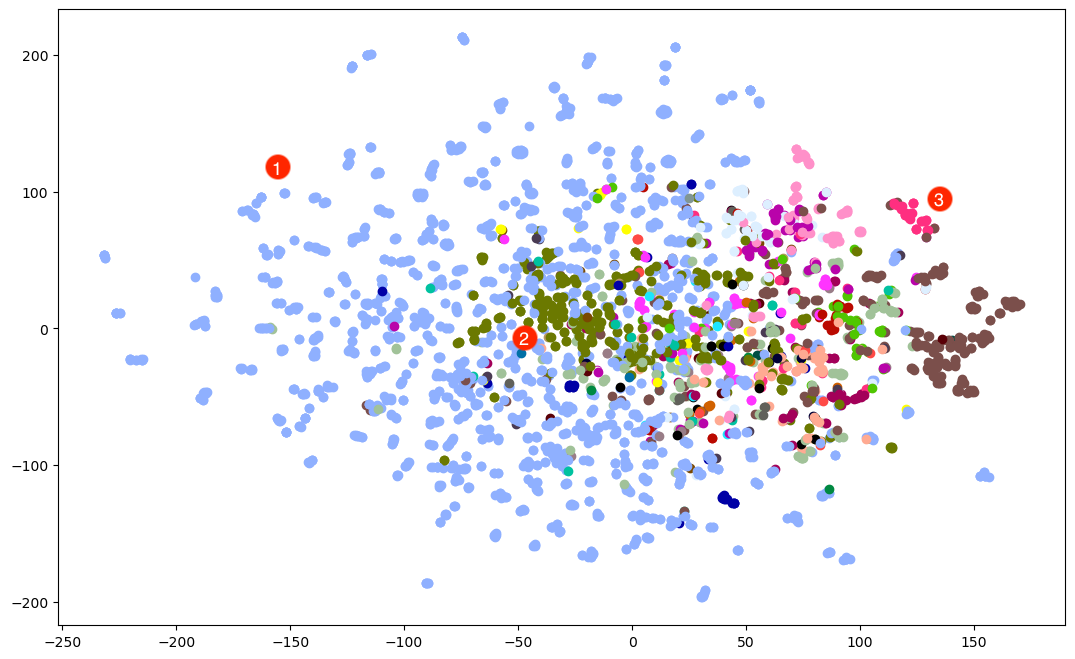
\includegraphics[width=11cm]{/Users/edoriggio/Documents/USI/github/thesis/research/out/plots/categories} }}%
    \qquad
    \subfloat[\centering Category Word Cloud] {{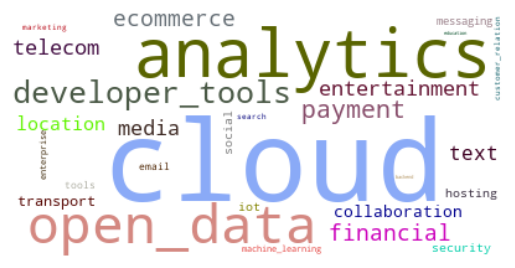
\includegraphics[width=6cm]{/Users/edoriggio/Documents/USI/github/thesis/research/out/plots/cloud} }}%
    \caption{APIs.guru Documents Plots}%
    \label{fig:documents-plot}%
\end{figure}
As we can see from both plots, the majority of the documents have been tagged with the \("\)cloud\("\) (\textbf{1}) and \("\)analytics\("\) (\textbf{2}) labels, even though most of them are not tightly clustered together.
Upon closer inspection, though, we can see that most -- if not all -- documents from the \("\)marketing\("\) (\textbf{3}) category are very close to one another.